%20 min preso!
\documentclass[xcolor=table,aspectratio=169]{beamer}
\usepackage{beamerthemesplit}
\usepackage{wrapfig}
\usetheme{SPbGU}
\usepackage{pdfpages}
\usepackage{amsmath}
\usepackage{cmap}
\usepackage[T2A]{fontenc}
\usepackage[utf8]{inputenc}
\usepackage[english]{babel}
\usepackage{indentfirst}
\usepackage{amsmath}
\usepackage{tikz}
\usepackage{multirow}
\usepackage[noend]{algpseudocode}
\usepackage{algorithm}
\usepackage{algorithmicx}
\usepackage{fancyvrb}
\usetikzlibrary{calc}
\usetikzlibrary{shapes,arrows}
\usetikzlibrary{arrows,automata}
\usetikzlibrary{positioning}
\usetikzlibrary{fit}
%\usepackage{caption}
\usepackage{subcaption}

\usepackage{kbordermatrix}
\renewcommand{\kbldelim}{(} 
\renewcommand{\kbrdelim}{)}

\newcommand\mca{\multicolumn{1}{c}{\cellcolor{red}\textbf{\{a\}}}}
\newcommand\mcb{\multicolumn{1}{c}{\cellcolor{red}\textbf{\{b\}}}}

\usepackage{tabularx}
\newcolumntype{Y}{>{\raggedleft\arraybackslash}X}

\renewcommand{\thealgorithm}{}

\newtheorem{mytheorem}{Theorem}
\renewcommand{\thealgorithm}{}

\newcommand{\tikzmark}[1]{\tikz[overlay,remember picture] \node (#1) {};}
\def\Put(#1,#2)#3{\leavevmode\makebox(0,0){\put(#1,#2){#3}}}

\newcommand{\ltz}{$< 1$}


\tikzset{
    state/.style={
           rectangle,
           rounded corners,
           draw=black, very thick,
           minimum height=2em,
           inner sep=2pt,
           text centered,
           },
}

\beamertemplatenavigationsymbolsempty

\title[All-Path CFPQ]{Context-Free Path Querying with All-Path Semantics by Matrix Multiplication}
%\subtitle[YaccConstructor]{Parsing techniques for graph analysis}
% То, что в квадратных скобках, отображается в левом нижнем углу.
\institute[JetBrains Research]{
JetBrains Research, Programming Languages and Tools Lab  \\
Saint Petersburg University
}

% То, что в квадратных скобках, отображается в левом нижнем углу.
\author[Rustam Azimov]{\textbf{Rustam Azimov}, Ilya Epelbaum, Semyon Grigorev }

\date{June 20, 2021}

\begin{document}
{
\begin{frame}[fragile]
  \begin{table}
  \centering
  \begin{tabularx}{\linewidth}{YcX}
    
\includegraphics[height=1.5cm]{pictures/jetbrainsResearch.pdf} \hfill
    & \begin{minipage}[t]{0.3\textwidth}\center \vspace{-1cm}  GRADES-NDA 2021
      \end{minipage}
    & \hfill 
\includegraphics[height=1.5cm]{pictures/SPbGU_Logo.png}
  \end{tabularx}
  \end{table}
  \titlepage
\end{frame}
}

\begin{frame} \frametitle{Context-Free Path Querying}
  \begin{minipage}[m]{0.45\linewidth}
  \raisebox{-0.5\totalheight}{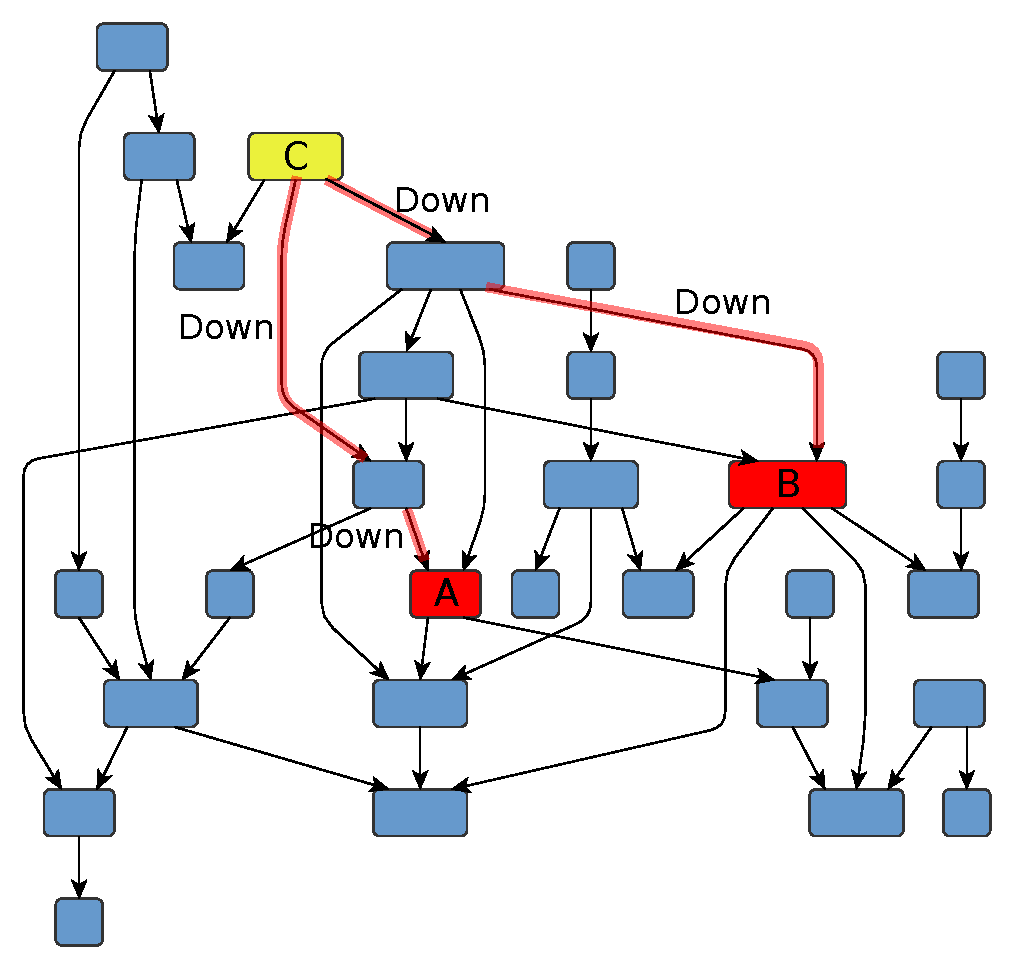
\includegraphics[width=\textwidth]{pictures/hierarchical.pdf}}
  \end{minipage}\hfill
  \begin{minipage}[m]{0.5\linewidth}
  \textbf{Context-free} languages as constraints on the paths
  \begin{itemize}
        \item Are nodes A and B on the same level of hierarchy?
        \item Is there a path of form $\overline{\textbf{Down}}^n \, \textbf{Down}^n$ between A and B?
        \item Find all paths of form $\overline{\textbf{Down}}^n \, \textbf{Down}^n$ between A and B
        
        \item Context-free grammar: $\textit{SameLvl} \to \overline{\textit{Down}} \ \textit{SameLvl} \ \textit{Down} \mid \varepsilon$
  \end{itemize}

  \end{minipage}

  \end{frame}

%  \begin{frame}[fragile] \frametitle{Applicatipons}
%    \begin{itemize}
%      \item Static code analysis
%      \item Graph database querying
%      \item RDF analysis
%    \end{itemize}
%  \end{frame}

  \begin{frame}[fragile]
    \frametitle{Context-Free Path Querying: Relational Query Semantics}
    \begin{itemize}
      \item $\mathbb{G} = (\Sigma, N, P)$ --- context-free grammar in normal form
      \begin{itemize}
        \item $A \rightarrow B C$, where $A, B, C \in N$
        \item $A \rightarrow x$, where $A \in N, x \in \Sigma \cup \{\varepsilon\}$
        \item $L(\mathbb{G},A) = \{ \omega \mid A \Rightarrow^* \omega \}$
      \end{itemize}
      \pause
      \item $G = (V,E,L)$ --- directed graph
        \begin{itemize}
          \item $v \xrightarrow{l} u \in E$
          \item $L \subseteq \Sigma$
        \end{itemize}
        \pause
      %\item $p = v_0 \xrightarrow{l_0} v_1 \xrightarrow{l_1} \cdots \xrightarrow{l_{n-2}} v_{n-1} \xrightarrow{l_{n-1}} v_n$ --- path in $G$
      \item $\omega(\pi) = \omega(v_0 \xrightarrow{l_0} v_1 \xrightarrow{l_1} \cdots \xrightarrow{l_{n-2}} v_{n-1} \xrightarrow{l_{n-1}} v_n) = l_0 l_1 \cdots l_{n-1}$
      \pause
      \item $R_A = \{ (n, m) \mid \exists n \pi m$, such that $\omega(\pi) \in L(\mathbb{G},A)\}$
    \end{itemize}
  \end{frame}

  \begin{frame}[fragile] \frametitle{Matrix-Based Algorithm: Relational Query Semantics}
    	\begin{algorithm}[H]
    		\begin{algorithmic}[1]
    			\caption{Context-free path querying algorithm}
    			\label{lst:algo1}
    			\Function{evalCFPQ}{$D=(V,E,L), G=(\Sigma,N,P)$}
    			\State{$n \gets$ |V|}
    			\State{$T \gets \{T^{A_i} \mid A_i \in N, T^{A_i}$ is a matrix $n \times n$, $T^{A_i}_{k,l} \gets$ \texttt{false}\} }
    			\ForAll{$(i,x,j) \in E$, $A_k \mid A_k \to x \in P$}
    			%\Comment{Matrices initialization}
    			%\For{$A_k \mid A_k \to x \in P$}
    			{$T^{A_k}_{i,j} \gets \texttt{true}$}
    			%\EndFor
    			\EndFor
    			\ForAll{$A_k \mid A_k \to \varepsilon \in P$}
    			\ForAll{$i \in \{0,\ldots ,n-1\}$}
    			{$T^{A_k}_{i,i} \gets \texttt{true}$}
    			\EndFor
    			\EndFor
    			
    			\While{any matrix in $T$ is changing}
    			%\Comment{Transitive c	losure calculation}
    			\For{$A_i \to A_j A_k \in P$}
    			{ $T^{A_i} \gets T^{A_i} + (T^{A_j} \times T^{A_k})$ } 
    			\EndFor
    			\EndWhile
    			\State \Return $T$
    			\EndFunction
    		\end{algorithmic}
    	\end{algorithm}
  \end{frame}


\begin{frame}[fragile]
\frametitle{Context-Free Path Querying: Single-Path Query Semantics}
\begin{itemize}
	\item For all $A \in N$, for all $(n,m) \in R_A$ also return some path $n\pi m$ such that $\omega(\pi) \in L(\mathbb{G},A)$
	\begin{itemize}
		\item usually the shortest path is returned
		\item returned path can be used as a proof of existence
	\end{itemize}
	\pause
	\item The main idea for the matrix-based algorithm is to store additional information in adjacency matrices to be able to restore one such path $n \pi m$ for all $(n,m) \in R_A$
	\begin{itemize}
		\item the intermediate vertex
		\item some additional information about path such as length
	\end{itemize}
	
\end{itemize}
\end{frame}

\begin{frame}[fragile]
	\frametitle{Context-Free Path Querying: All-Path Query Semantics}
	\begin{itemize}
		\item For all $A \in N$, for all $(n,m) \in R_A$ also return \textbf{all} paths $n\pi m$ such that $\omega(\pi) \in L(\mathbb{G},A)$
		\begin{itemize}
			\item in some cases we want to find all data dependencies, for example in static code analysis when searching for vulnerabilities
			\item the number of such paths can be infinite if the input graph has cycles
		\end{itemize}
		\pause
		\item Currently, our matrix-based algorithms cannot handle the all-path query semantics
		
		\item The only linear algebra-based algorithm that solves this problem is the Kronecker product-based CFPQ algorithm
		
	\end{itemize}
\end{frame}


\begin{frame}[fragile] \frametitle{Research Questions}
\begin{itemize}
	\item Can we extend the matrix-based CFPQ algorithm to all-path query semantics?
	\item What the cost of such extension?
	\item How does the matrix-based solution for the all-path query semantics compare to the Kronecker product-based?
\end{itemize}
\end{frame}

\begin{frame}[fragile] \frametitle{All-Path Index}
\begin{itemize}
	\item We store the additional information about the paths found as the sets of the intermediate vertices
	\item We introduce the following matrix multiplication operation
	\item $T^A \odot T^B = T^C$ where $T^C_{i,j} = \bigcup^{n}_{k = 1} (T^A_{i,k} \otimes T^B_{k,j})$ and  
\end{itemize}
$$T^A_{i,k} \otimes T^B_{k,j} = \begin{cases} \{k\}, & \mbox{if } T^A_{i,k} \neq \emptyset \wedge T^B_{k,j} \neq \emptyset \\ \emptyset, & \mbox{otherwise} \end{cases}$$
\end{frame}

 

 % \begin{frame}[fragile] \frametitle{Matrix-Based Algorithm: Technical Details}
  %  \begin{itemize}
   %   \item We can remove $\textit{length}$ or $\textit{height}$ to reduce memory consumption
    %  \item The PathIndex operations can be represented as bitwise atomic operations
     % \item We still can use existing high-performance libraries for matrix operations if they support the creation of custom operations
    %\end{itemize}
  %\end{frame}


%\begin{frame}[fragile] \frametitle{Example: Graph and Grammar}
%  	\[
%  	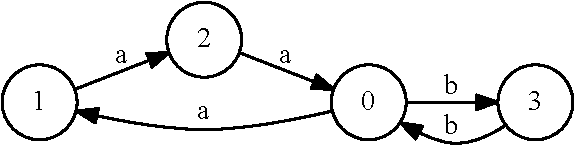
\includegraphics[width=5cm]{pictures/example_graph.pdf}
%  	\]
%  	\pause
%  	\[
%  	\begin{array}{rcclcrccl}
%  	0: & S & \rightarrow & A \ B   & \quad & 3: & A & \rightarrow & \text{\emph{a}}     \\
%  	1: & S & \rightarrow & A \ S_1       & \quad & 4: & B & \rightarrow & \text{\emph{b}} \\
%  	2: & S_1 & \rightarrow & S \ B & & & & &
%  	
%  	\end{array}
%  	\]
%  	
%\end{frame}

%\begin{frame}[fragile] \frametitle{Example: Initial Matrices}
%\[
%T^{(1),A} = \begin{pmatrix}
%\bot & (0,1,0,1,1)       & \bot & \bot       \\
%\bot & \bot & (1,2,1,1,1)       & \bot \\
%(2,0,2,1,1)       & \bot & \bot & \bot \\
%\bot       & \bot & \bot & \bot \\
%\end{pmatrix}
%\]
%\[
%T^{(1),B} = \begin{pmatrix}
%\bot & \bot       & \bot & (0,3,0,1,1)       \\
%\bot & \bot & \bot       & \bot \\
%\bot       & \bot & \bot & \bot \\
%(3,0,3,1,1)      & \bot & \bot & \bot \\
%\end{pmatrix}
%\]
%
%\end{frame}

%\begin{frame}[fragile] \frametitle{Example: Final Matrix}
%\[
%T^{(14),S} = \begin{pmatrix}
%(0,0,1,12,12) & \bot       & \bot & (0,3,1,6,6)       \\
%(1,0,2,4,4) & \bot & \bot       & (1,3,2,10,10) \\
%(2,0,0,8,8)       & \bot & \bot & (2,3,0,2,2) \\
%\bot       & \bot & \bot & \bot \\
%\end{pmatrix}
%\]
%
%\end{frame}

%\begin{frame}[fragile] \frametitle{Path Extraction Algorithm}
%\begin{algorithm}[H]
%	\begin{algorithmic}[1]
%		\caption{Path extraction algorithm}
%		\label{lst:algo3}
%		\Function{extractPath}{$i, j, A, T=\{T^{A_i}\}, G=(N,\Sigma,P)$}
%		\State{$index \gets T^{A}_{i,j}$ }
%		
%		\If{$index = \bot$}
%		\State \Return $\pi_{\emptyset}$
%		\Comment{Such a path does not exist}
%		\EndIf
%		
%		\If{$index.height = 1$}
%		\If{$index.length = 0$}
%		\State \Return $[]$
%		\Comment{Return an empty path}
%		\EndIf
%		\ForAll{$ x \mid (i,x,j) \in E$}
%		\If{$A \to x \in P$}
%		\State \Return $[(i,x,j)]$
%		\Comment{Return a path of length one}
%		\EndIf
%		\EndFor
%		\EndIf
%		
%		\ForAll{$A \to B C \in P$}
%		\State{$index_B \gets T^{B}_{i,index.middle}$ }
%		\State{$index_C \gets T^{C}_{index.middle,j}$ }			
%		\If{$(index_B \neq \bot) \wedge (index_C \neq \bot)$}
%		\State{$maxH \gets max(index_B.height, index_C.height)$ }
%		\If{$index.height = maxH + 1$}
%		
%		
%		\State{$\pi_1 \gets$ \Call{extractPath}{$i, index.middle, B, T, G$}}
%		\State{$\pi_2 \gets$ \Call{extractPath}{$index.middle, j, C, T, G$}}
%		\State \Return $\pi_1 + \pi_2$
%		\Comment{Return the concatenation of paths}
%		\EndIf
%		\EndIf
%		\EndFor
%		\EndFunction
%	\end{algorithmic}
%\end{algorithm}
%\end{frame}


\begin{frame}[fragile] \frametitle{Path extraction}

\begin{itemize}
	\item After constructing a set of matrices with sets of intermediate vertices, we can extract all required paths $i\pi j$ for every vertex pair $i, j$ if such paths exist
	\item It is	assumed that the sets of paths are computed lazily, to ensure the	termination in case of an infinite number of paths
	
\end{itemize}
\end{frame}


\begin{frame}[fragile] \frametitle{Implementation}

\begin{itemize}
	\item For evaluation we use the following CPU-based implementations of CFPQ algorithms with sparse matrix representation
	\begin{itemize}
		\item \textbf{$MtxRel$} --- for  relational query semantics that uses \textbf{pygraphblas} --- a Python wrapper around the GraphBLAS API
		\item \textbf{$MtxSingle$} --- for  single-path query semantics that also uses \textbf{pygraphblas}
		\item \textbf{$MtxAll$} --- the implementation of the proposed matrix-based algorithm for all-path query semantics which utilizes \textbf{SuiteSparse} and our own Python wrapper
		\item \textbf{$Tns$} --- the implementation of the Kronecker product-based algorithm for all-path query semantics that uses \textbf{pygraphblas}
		
	\end{itemize}
\end{itemize}
\end{frame}


\begin{frame} \frametitle{Evaluation Setup}
  \begin{itemize}
  	\item Ubuntu 18.04, Intel Core i7-6700 CPU, 3.4GHz, DDR4 64Gb RAM
  	\item We use graphs corresponding to real RDFs
  	\item We use same-generation query
  \end{itemize}
\end{frame}

\begin{frame}[fragile] \frametitle{Evaluation: CFPQ\footnote{Time in seconds and memory is measured in megabytes}}
\begin{center}
	\tikzmark{yyy}{
	}
	{\scriptsize
	{\setlength{\tabcolsep}{0.3em}
			\rowcolors{3}{}{lightgray}
					\begin{tabular}{|l|l|l|l|l|l|l|l|l|l|l|}
						\hline
						\multicolumn{1}{|c|}{\multirow{2}{*}{Graph}} & \multicolumn{1}{c|}{\multirow{2}{*}{\#V}} & \multicolumn{1}{c|}{\multirow{2}{*}{\#E}} &  \multicolumn{2}{c|}{MtxRel} & \multicolumn{2}{c|}{MtxSingle} & \multicolumn{2}{c|}{MtxAll} & \multicolumn{2}{c|}{Tns} \\ \cline{4-11} 
						\multicolumn{1}{|c|}{}                       & \multicolumn{1}{c|}{}                     & \multicolumn{1}{c|}{}                     & Time         & Mem          & Time        & Mem        & Time           & Mem           & Time         & Mem    \\ \hline
						pathways                                     & 6 238                                     & 18 598 & 0.01         & 140  & 0.01           & 671 & 0.01         & 49           & 0.01        & 122               \\ \hline
						go-hierarchy                                 & 45 007                                    & 980 218                                   & 0.09         & 255 & 0.84           & 671 & 0.35        & 195        & 0.24        & 252                             \\ \hline
						enzyme                                       & 48 815                                    & 109 695                                   & 0.01         & 181 & 0.01           & 217 & 0.02         & 61           & 0.02        & 132                            \\ \hline
						eclass\_514en                                & 239 111                                   & 523 727                                   & 0.06         & 181 & 0.16           & 216    & 0.22         & 126          & 0.27        & 193                         \\ \hline
						go                                           & 272 770                                   & 534 311                                   & 0.94         & 246  & 0.93           & 217  & 1.13         & 990          & 1.27        & 243                          \\ \hline
						%geospecies                                   & 450 609                                   & 2 311 461                   & 0.01         & 248 & 0.01           & 2251            & 0.34         & 156          & 0.01        & 196              \\ \hline
						geospecies & 450 609                                   & 2 311 461 & 7.48         & 7645     & 15.54          & 22941 & 32.06        & 44235        & 26.32       & 19537 \\ \hline
						taxonomy                                     & 5 728 398                                 & 14 922 125                            & 0.72         & 1175      & 1.15           & 2250    & 3.84        & 1507        & 3.56        & 1776                   \\ \hline
					\end{tabular}
	}
}
 \end{center}
\pause
\onslide<2>{\tikz[overlay,remember picture]{\draw[draw=red,thick,fill opacity=0.2] ($ (yyy) + (5.22,-0.41)$) rectangle ($ (yyy) + (8.78,-1.53)$);}}
\pause
\onslide<3>{\tikz[overlay,remember picture]{\draw[draw=red,thick,fill opacity=0.2] ($ (yyy) + (6.88,-0.41)$) rectangle ($ (yyy) + (10.58,-1.53)$);}}
\pause
\onslide<4>{\tikz[overlay,remember picture]{\draw[draw=red,thick,fill opacity=0.2] ($ (yyy) + (8.69,-0.41)$) rectangle ($ (yyy) + (12.40,-1.53)$);}}
\end{frame}

\begin{frame}[fragile] \frametitle{Evaluation: Average Path Extraction Time For \textit{go}}
\begin{center}
    \[
		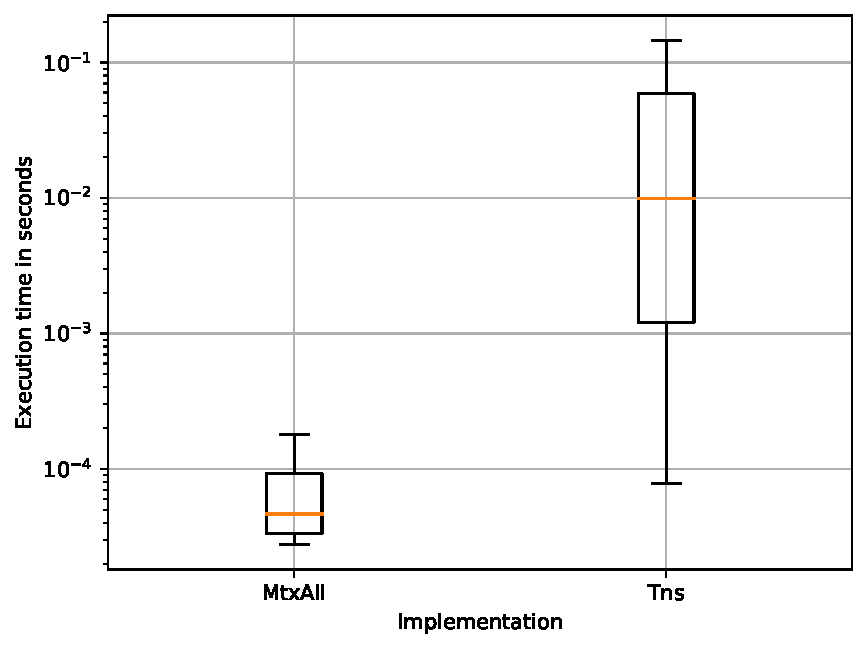
\includegraphics[width=9cm]{pictures/go_10_all_matrixall_tensor.pdf}
	\]
\end{center}

\end{frame}

\begin{frame}[fragile] \frametitle{Evaluation Results}
	\begin{itemize}
		\item The proposed algorithm constructs index up to 2-3 times slower and consumes more memory than the algorithm for single-path query semantics
		\pause
		\item If it is necessary to frequently recalculate
		the index for a changing graph or a path query then the best
		choice is the Kronecker product-based algorithm with
		faster and less memory consuming index construction
		\pause
		\item If it is  necessary to extract paths many times for a once constructed
		index or index changes can be efficiently computed dynamically then the proposed matrix-based CFPQ algorithm is  preferable
	\end{itemize}
	%\pause
	%\begin{itemize}
	% \item Dataset is published: both graphs and queries
	%\begin{itemize}
	%	\item Link: \url{https://github.com/JetBrains-Research/CFPQ_Data}
	%\end{itemize}
	
	%\item Implementations are available on GitHub
	%\begin{itemize}
	%	\item Link: \url{https://github.com/JetBrains-Research/CFPQ_PyAlgo}
	%\end{itemize}
	
	%\end{itemize}
\end{frame}

\begin{frame}[fragile] \frametitle{Conclusion}
  \begin{itemize}
    \item The matrix-based CFPQ algorithm can be extended for all-path query semantics
    \pause
    \item The cost of such extension is an increase in the index creation time and a large increase in memory consumption for some graphs and queries with complex structure of result
    \pause
    \item The proposed matrix-based solution for all-path query semantics compared to the Kronecker product-based solution consumes more memory, but allows one to extract paths significantly faster 
  \end{itemize}
  %\pause
  %\begin{itemize}
   % \item Dataset is published: both graphs and queries
    %\begin{itemize}
    %	\item Link: \url{https://github.com/JetBrains-Research/CFPQ_Data}
    %\end{itemize}
    
    %\item Implementations are available on GitHub
    %\begin{itemize}
    %	\item Link: \url{https://github.com/JetBrains-Research/CFPQ_PyAlgo}
    %\end{itemize}
    
  %\end{itemize}
\end{frame}

\begin{frame}[fragile] \frametitle{Future Research}
  \begin{itemize}
  	\item We compare the CPU-based implementation. In the future, we
  	want to obtain GPU-based and distributed implementations 
  	\item Also, further improvements in index creation and path extraction
  	for both matrix-based and Kronecker product-based algorithms are
  	required
    \item We plan to provide the multiple-source
    modifications for all linear algebra-based CFPQ algorithms
\end{itemize}
\end{frame}

\begin{frame}
\frametitle{Contact Information}
\begin{itemize}
  \item Semyon Grigorev:
    \begin{itemize}
      \item \href{mailto:s.v.grigoriev@spbu.ru}{s.v.grigoriev@spbu.ru}
      \item \href{mailto:Semen.Grigorev@jetbrains.com}{Semen.Grigorev@jetbrains.com}
    \end{itemize}
  \item Rustam Azimov:
  \begin{itemize}
  	\item \href{mailto:rustam.azimov19021995@gmail.com}{rustam.azimov19021995@gmail.com}
  	\item \href{mailto:Rustam.Azimov@jetbrains.com}{Rustam.Azimov@jetbrains.com}
  \end{itemize}
  \item Ilya Epelbaum: \href{mailto:iliyepelbaun@gmail.com}{iliyepelbaun@gmail.com}
\vspace{0.5cm}
  \item Dataset: \href{https://github.com/JetBrains-Research/CFPQ_Data}{https://github.com/JetBrains-Research/CFPQ\_Data}
   \item Algorithm implementations: \href{https://github.com/JetBrains-Research/CFPQ_PyAlgo}{https://github.com/JetBrains-Research/CFPQ\_PyAlgo}
\end{itemize}
\vspace{0.1cm}
\center{\huge{Thanks!}}
\end{frame}
\end{document}
